\documentclass{article}\usepackage[]{graphicx}\usepackage[]{color}
%% maxwidth is the original width if it is less than linewidth
%% otherwise use linewidth (to make sure the graphics do not exceed the margin)
\makeatletter
\def\maxwidth{ %
  \ifdim\Gin@nat@width>\linewidth
    \linewidth
  \else
    \Gin@nat@width
  \fi
}
\makeatother

\definecolor{fgcolor}{rgb}{0.345, 0.345, 0.345}
\newcommand{\hlnum}[1]{\textcolor[rgb]{0.686,0.059,0.569}{#1}}%
\newcommand{\hlstr}[1]{\textcolor[rgb]{0.192,0.494,0.8}{#1}}%
\newcommand{\hlcom}[1]{\textcolor[rgb]{0.678,0.584,0.686}{\textit{#1}}}%
\newcommand{\hlopt}[1]{\textcolor[rgb]{0,0,0}{#1}}%
\newcommand{\hlstd}[1]{\textcolor[rgb]{0.345,0.345,0.345}{#1}}%
\newcommand{\hlkwa}[1]{\textcolor[rgb]{0.161,0.373,0.58}{\textbf{#1}}}%
\newcommand{\hlkwb}[1]{\textcolor[rgb]{0.69,0.353,0.396}{#1}}%
\newcommand{\hlkwc}[1]{\textcolor[rgb]{0.333,0.667,0.333}{#1}}%
\newcommand{\hlkwd}[1]{\textcolor[rgb]{0.737,0.353,0.396}{\textbf{#1}}}%

\usepackage{framed}
\makeatletter
\newenvironment{kframe}{%
 \def\at@end@of@kframe{}%
 \ifinner\ifhmode%
  \def\at@end@of@kframe{\end{minipage}}%
  \begin{minipage}{\columnwidth}%
 \fi\fi%
 \def\FrameCommand##1{\hskip\@totalleftmargin \hskip-\fboxsep
 \colorbox{shadecolor}{##1}\hskip-\fboxsep
     % There is no \\@totalrightmargin, so:
     \hskip-\linewidth \hskip-\@totalleftmargin \hskip\columnwidth}%
 \MakeFramed {\advance\hsize-\width
   \@totalleftmargin\z@ \linewidth\hsize
   \@setminipage}}%
 {\par\unskip\endMakeFramed%
 \at@end@of@kframe}
\makeatother

\definecolor{shadecolor}{rgb}{.97, .97, .97}
\definecolor{messagecolor}{rgb}{0, 0, 0}
\definecolor{warningcolor}{rgb}{1, 0, 1}
\definecolor{errorcolor}{rgb}{1, 0, 0}
\newenvironment{knitrout}{}{} % an empty environment to be redefined in TeX

\usepackage{alltt}
%\usepackage{animate}
\usepackage[round]{natbib}
%\usepackage[nolists]{endfloat}
\usepackage[width = 5in]{geometry}
\usepackage{pdfpages, caption}
\usepackage{rotating}
\usepackage{caption, amsmath, graphicx, setspace, multirow, color, hyperref, array}
\usepackage{xcolor, colortbl}
\usepackage{arydshln}

\definecolor{Gray}{gray}{0.85}
\definecolor{Gray95}{gray}{0.95}
\definecolor{Gray75}{gray}{0.75}

\title{Can Conventional Measures Identify Geographically Varying Mixed Regression Relationships? A Simulation-based Analysis of Locally Weighted Regression}
\author{Aaron Swoboda}
\IfFileExists{upquote.sty}{\usepackage{upquote}}{}
\begin{document}
\maketitle





\tableofcontents
\listoffigures
\listoftables

\section{Background}

Imagine a simple linear model,
\begin{equation}\label{eq:simpleOLS}
Y = \beta _0 + \beta _1 *X_1 + \beta _2 * X_2 + \epsilon .
\end{equation}
In addition to the three variables listed above ($Y$, $X_1$, and $X_2$), assume we know the geographical location for each of our $N$ observations. Thus, our data consists of an $N \times 5$ matrix, where $Y$ may be house prices, $X_1$ and $X_2$ could be the living space and lot size associated with each house, and the final two columns determine the location of the observations (for instance, latitude and longitude, or distances north and east from a prescribed point).

The simple model in \eqref{eq:simpleOLS} exemplifies spatial stationarity in the parameters: the $\beta$ coefficients are constant over space. Alternatively, the coefficients could exhibit spatial non-stationarity, in which case one, two, or all three of the $\beta$ coefficients vary with location. This has a natural interpretation in the current real estate example: location matters. However, location can matter in different ways. For instance, if the value of land varies over space, then we would expect the coefficient on lot size to vary over space, while it is also possible that the intercept varies over space to reflect variation in prices of similar houses in different locations. 

It is possible to parameterize the variation in coefficients, for instance by including a variable measuring the distance from an observation to an important amenity such as the Central Business District and then this distance variable could be interacted with variables whose value are predicted to vary over space. However, it is plausible that the variation in coefficients might not be easily parameterized (for instance, if land values are a non-monotonic function of distance). Researchers may instead interact variables with fixed effects for cities or census tracts. However, such strategies require the analyst to make assumptions that severely limit the type and degree of variation in the parameters. For instance, interaction terms with geographic boundaries assume discrete differences in the value of parameters across the boundaries, while instead the parameters may instead be a continuous function of location. Additionally, numerous interaction terms may unduly reduce the degrees of freedom.

\subsection{Weighted Regression to the Rescue?}
Locally Weighted Regression (LWR) techniques are one set of potential solutions to the challenge described. It is a weighted least squares methodology in which regression coefficients are estimated as a function of the local data. \citet{Cleveland1988} provides one of the first descriptions of the method, while more recently \citet{Brunsdon1998b} and \citet{Fotheringham2002} have explicitly incorporated geography/location into the methodology. Specifically, the coefficients are estimated,
\begin{equation}\label{eq:LWRbeta}
\hat{\beta}(location_i) = (X'W(location_i)X)^{-1}X'W(location_i)Y,
\end{equation}
where X is a $N \times m$ matrix of independent variables, $W_i$ is the $N \times N$ weights matrix, and Y is the $N \times 1$ vector of dependent variable values. The weights matrix, $W_i$ is a diagonal matrix where element $w_{jj}$ denotes the weight that the $j^{th}$ data point will receive in the regression coefficients estimated at location $i$ in the dataset.\footnote{If all diagonal elements of $W$ are one, then \eqref{eq:LWRbeta} simplifies to the standard OLS estimation.} We employ a bi-square weights function and a k-nearest neighbor bandwidth approach as described in equation~\eqref{eq:weights}, 
\begin{equation}\label{eq:weights}
w_{jj}=\left[1-\left(\frac{d_{ij}}{d_{k}}\right)^2 \right]^2 \textrm{ if }d_{ij}<d_{ik}\textrm{, otherwise = 0},
\end{equation}
where $d_{ij}$ denotes the distance between observations $i$ and $j$, and $d_{ik}$ is the distance from observation $i$ to the $k^{th}$ nearest observation. This function assigns weights close to 1 for data points near observation $i$, weights positive but closer to zero for observations farther away, and zero for all $n-k$ observations farther away than the $k^{th}$ nearest observation. 

A key decision in estimating LWR models is choosing the number of observations to include in the bandwidth. Bandwidths that are too large in the presence of spatial non-stationarity create bias in the regression estimates (the large bandwidth creates weights matrices that are similar over space and therefore the regression coefficients are forced to be similar when they should vary over space). Bandwidths that are too small add unneccessary error in our estimates by excluding informative observations. Often, researchers choose a bandwidth my minimizing a cross validation metric. 

\subsection{Mixed Geographic Models}

Thus far two models have been discussed - the standard OLS model in which all of the coefficients are stationary and a local model in which all coefficients are estimated locally using some bandwidth. The two cases are identical in the extreme case of an infinite bandwidth. Other ``mixed'' models are also possible in which some coefficients are assumed to be stationary while others are estimated locally. 

This choice of bandwidth is further complicated in the context of mixed models where only some coefficents exhibit spatial stationarity (in contrast to standard models in which all coefficients are treated as spatially stationary or LWR models in which no coefficients are treated as stationary). In this case, researchers must choose which variables to treat as spatially non-stationary and the bandwidth at which to perform the analysis. Little is known about model performance when models are selected across multiple mixed models and among multiple different potenial bandwidth sizes. This paper uses simulated data generated under multiple conditions to begin to answer some of the outstanding questions in the area of geographically mixed models. 



\subsection{Model Selection}

Gotta say something about \citet{Leung2000a}. What does it do and what are some potential weaknesses?

They talk about two things... first develop a test of stationarity for the model as a whole, then a step-wise model for adding/subtracting spatially varying variables. Weaknesses? Some quote about "not being able to undo" the addition or subtraction, which may be a problem in the presence of correlated coefficients.

The \citet{Fotheringham2002} text suggests a system of Monte Carlo experiments.


We compare four important cross-validation/information criteria: Leave One Out Cross Validation (LOOCV), Generalized Cross Validation (GCV), Standardized Cross Validation (SCV), and the Akaike Information Criterion (AIC). How frequently can researchers utilizing these metrics identify the correct model among the various possible combinations? Are certain metrics more/less prone to false positive/negatives? Do they suggest no spatial variation when in fact it exists? Do they suggest spatial variation when in fact there is not? 

\subsubsection{Leave One Out Cross Validation}
Perhaps the most common cross validation metric used in the literature is the Leave One Out Cross Validation score (LOOCV), which is calculated as follows,
\begin{equation}\label{eq:LOOCV}
LOOCV = \frac{1}{N} \sqrt{\sum _{i = 1}^{N} (y - \hat{y}_{\neq i})^2},  
\end{equation}
where $\hat{y}_{\neq i}$ represents the dependent variable estimate for observation $i$ while excluding observation $i$ from the regression. This prevents the observation from having undue influence in the regression with small bandwidths and overfitting the model. Such a model, while intuitively appealing, can be computationally expensive, as regressions must be estimated first while excluding individual observations to calculate the LOOCV and then again while including the observation to obtain the regression coefficients.

\subsubsection{Generalized Cross Validation}
An alternative cross validation metric is known as the Generalized Cross Validation (GCV) score, which only requires calculating the regressions once per location and explicitly calculates the leverage each observation has over the regression coefficients. The GCV score calculation is detailed in equation~\eqref{eq:GCV},
\begin{equation}\label{eq:GCV}
n*\sum_{i=1}^{n}\frac{(y_i-\hat{y}_i)^2}{(n-v_1)^2}, 
\end{equation} 
where $\hat{y}_i$ is the predicted dependent variable value for observation $i$, and $v_1$ can be interpreted as the ``effective number of model parameters,'' and calculated as $v_1=$tr(\textbf{S}), where the matrix \textbf{S} is the ``hat matrix'' which maps $y$ onto $\hat{y}$,
                   \begin{equation}
                   \hat{y}=\textbf{S}y,
                   \end{equation}
                   and each row of \textbf{S}, $r_i$ is given by:
                  \begin{equation}
                   r_i=X_i(X'W_iX)^{-1}X'W_i.
                   \end{equation}
The GCV score is a convenient model selection metric that rewards models that provide a good fit to the data, while penalizing models with a greater number of model parameters \citep{Loader1999, McMillen2010}.  \citep{Paez2011, McMillen2010, McMillen2012}. 

\subsubsection{Standardized Cross Validation}
The Standardized Cross Validation Score was suggested by \citep{Farber2007b} and elaborated on in \citep{Paez2011} as an alternative to conventional metrics. This metric is designed to limit the influence of outliers which may disproportionately impact the choice of bandwidth. The Standardized Cross Validation score for a given observation $i$ and bandwidth $k$ is, 
\begin{equation}\label{eq:SCV}
SCV_i (k) = \frac{\sum (y_i - \hat{y}_{-i}(k))^2} {\sum _k (y_i - \hat{y}_{-i})^2 },
\end{equation}
and the total score for bandwidth $k$ is then,
\begin{equation}\label{eq:SCVtot}
SCV(k) = \sum _i SCV_i(k).
\end{equation}
Equation \eqref{eq:SCV} calculates a partial score for each observation as a proportion of the total squared deviance at that observation across the different bandwidths, while \eqref{eq:SCVtot} then calculates the sum across all observations for a given bandwidth. Note that, contrary to the other metrics described here, the SCV score has to be calculated after all possible bandwidths have been implemented.

\subsubsection{Akaike Information Criterion}
As noted in \citep{Fotheringham2002}, the well-known Akaike Information Criterion is calculated in the geographically weighted regression framework as follows,
\begin{equation}\label{eq:AIC}
  2*n*ln(\hat{\sigma}) + n*ln(2*\pi) + 
    n*\frac{n + v_1}{n - 2 - v_1}
    \end{equation}
where $\hat{\sigma}$ is the estimated standard error of the regression, n is the sample size, and $v_1$ remains the ``effective number of parameters'' estimated by the model as described above.


\subsection{Examples of citations using different methods...}
\subsubsection{Uses the AIC}
\cite{Borst2007}
\citet{Axhausen2010}
\citet{Cahill2007}
\citet{Eckey2007}
\citet{Foody2003}
\citet{Hanink2010}
\citet{Haynes2011}
\citet{Helbich2009}
\citet{Kestens2005}
\citet{Partridge2008}
\citet{Partridge2007}
\citet{PinedaJaimes2010}
\citet{Sa2010}
\citet{Tu2008}
\citet{Yu2006}
\citet{Yu2007a}
\citet{Yu2007}

\subsection{Uses SCV}
No one in our sample, but do a google scholar search and look for articles that cite the original articles

\begin{verbatim}
\https://scholar.google.com/scholar?as_ylo=2011&hl=en&as_sdt=5,24&sciodt=0,24&cites=9654495652239805234&scipsc=
\end{verbatim}

\subsection{Uses LOOCV}
\citet{Brunsdon1998}
\citet{Cho2006a}
\citet{Cho2009}
\citet{Huang2002}
\citet{Lloyd2005}
\citet{Lloyd2005}
\citet{Lloyd2005}
\citet{Lloyd2005}

\subsubsection{Mixed Models?}

\citet{Cahill2007} determine that a mixed model might be best because of Monte Carlo simulations.

\citet{Huang2010} find evidence consistent with a mixed model (some coefficients appear to stationary and others non-stationary), but do not estimate one.

\citet{Yu2006} implement a mixed model after using tests of spatial stationarity 

\citet{Chow2000} uses the AIC to select which variables are nonstationary.

\citet{Mei2004} seems like an important article to talk about. It proposes a methodology for selecting a mixed model. Google Scholar has info on who cites this article.
\begin{verbatim}
https://scholar.google.com/scholar?cites=11649932945261630952&as_sdt=5,24&sciodt=0,24&hl=en
\end{verbatim}


\subsection{Experimental Design}

For a given sample size, $n \in \{50, 100, 200, 800\}$ we generate an $n \times 4$ matrix of  uniformly independently distributed values between 0 and 1. Let the first two of these columns be called $East$ and $North$ and denote the location of each of our observations within a two-dimensional unit grid (East, North), while the remaining two columns be $X_1$ and $X_2$ and serve as the independent variables in our regression equation.

Our goal is to generate data according to the following process:
\begin{equation} \label{eq:DGP}
Y_i = \beta _0 (East_i, North_i) + \beta _1 (East_i, North_i)*X_{1i} + \beta _2 (East_i, North_i) * X_{2i} + \epsilon _i ,
\end{equation}
where $\epsilon _i n(0, \sigma ^2)$. Equation \ref{eq:DGP} states that the dependent variable value for a given observation depends on the values of $X_1$, $X_2$, a normally distributed error term, and the values of three $\beta$ coefficients, each of which is a function of the location within our dataset.

The relationship between location and $\beta _1$ is given by,
\begin{equation}\label{eq:beta1}
\beta _1 =  2 + \eta _1 \times (East - .5) ,
\end{equation}
where the $\eta _1$ parameter changes the degree to which the $\beta _1$ coefficient varies over space. When $\eta _1 =0$, equation \eqref{eq:beta1} simplifies to $\beta _1 =2$ and there is no spatial variation in the coefficient. When $\eta _1 \in \{1, 2\}$, there is a linear relationship between $\beta _1$ and the $East$ location of the data point. Note that the expected value of $\beta _1 = 2$ for all three cases of $\eta _1 \in \{0, 1, 2\}$ because of the uniform distribution of $East \in [\, 0, 1]\,$. A visual representation of the relationship is presented in the first row of Figure \ref{fig:spvarBeta}.

Similar to $\beta _1$, the relationship between location and $\beta _2$ is given by,
\begin{equation}\label{eq:beta2}
\beta _2 =  2 + \eta _2 \times (North- .5),
\end{equation}
where the $\eta _2$ parameter changes the degree to which the $\beta _2$ coefficient varies over space. When $\eta _2 =0$, equation \eqref{eq:beta2} simplifies to $\beta _2 =2$ and there is no spatial variation in the coefficient. When $\eta _2 \in \{1, 2\}$, there is a linear relationship between $\beta _2$ and the $North$ location of the data point. Note that the expected value of $\beta _2 = 2$ for all three cases of $\eta _2 \in \{0, 1, 2\}$ because of the uniform distribution of $North \in [\, 0, 1]\,$. A visual representation of the relationship is presented in the second row of Figure \ref{fig:spvarBeta}.

The $\beta _1$ and $\beta _2$ coefficients are orthogonal to one another ($\beta 1$ is a function of the $East$ locational variable, while $\beta _2$ is a function of $North$.) In order to introduce spatial non-stationarity in the $\beta _0$ coefficient without also creating high and/or perfect multicollinearity among the coefficients, we generated the $\beta _0$ coefficient by the following,
\begin{equation}\label{eq:beta0}
\beta _0 = 2 + \eta _0 \times \Bigg[C + cos\Bigg(2\pi\times\sqrt{\frac{(East - .5)^2 + (North- .5)^2}{.5}}\Bigg)\Bigg],
\end{equation}
where $C$ is a constant selected to yield an $E(\beta _0) = 2$. Equation \eqref{eq:beta0} is presented visually in the third row of Figure \ref{fig:spvarBeta}.


\begin{figure}
\makebox[\textwidth][c]{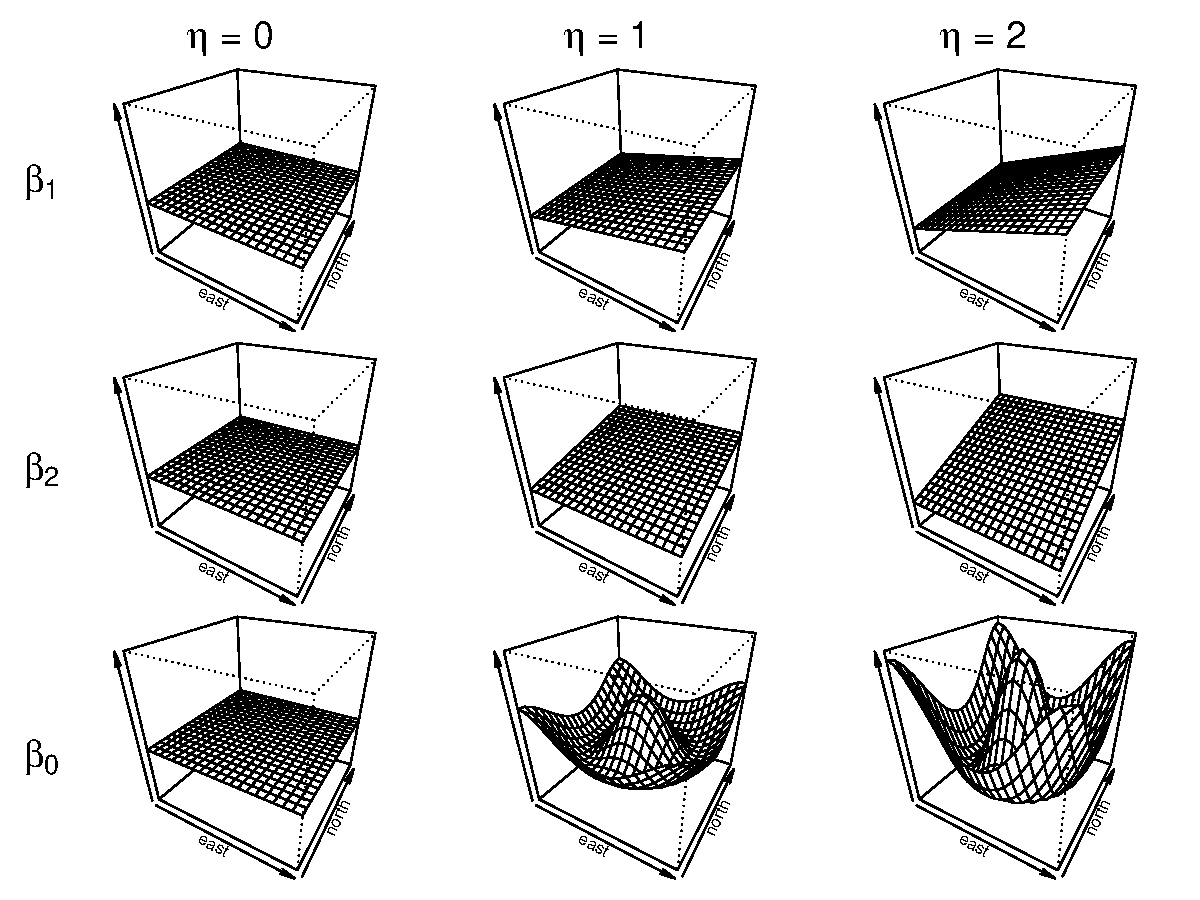
\includegraphics[width = 1.1\textwidth]{SpatialVariationBetas}}
\caption{Visual Representation of the Spatial Variation for the Three Coefficientsas Described in Equations \eqref{eq:beta1} - \eqref{eq:beta0}}
\label{fig:spvarBeta}
\end{figure}


% We write $\beta _m (East, North)$, $m = \{0, 1, 2\}$, to denote that each of the three coefficients may vary over space (they are spatially non-stationary). If all three coefficients are instead stationary, $\beta _m(location) = \beta _m$, then Equation \ref{eq:DGP} is simply a standard regression equation and the three coefficients could be estimated using Ordinary Least Squares. 
% 
% We generate each of the $\beta _m$ coefficient vectors according to three different scenarios. First, we assume spatial stationarity in which each coefficient is equal to 2. We also generate each $\beta _m$ coefficient with \emph{some} spatial non-stationarity and \emph{more} non-stationarity. 
% 
% and other times it is non-stationary, $\beta _m (location_p) \neq \beta _m (location_q)$. With three coefficients each having the possibility of being stationary or not, there are eight different possible combinations of the three parameters, ranging from (stationary, stationary, stationary) to (non-stationary, non-stationary, non-stationary). We refer to any parameter combination containing both stationary and non-stationary coefficients as ``mixed.''
% 
% We generate data using all eight different combinations and then estimate all eight possible LWR models across seven different bandwidth sizes. We then calculate different Cross-Validation metrics and compare their values across models and bandwidths. 
% 
% We have three different values for each coefficient in our DGP, no variation, some variation, and more variation. We also change the sample size of our data as well as the variance of the model error term.
% 
% The following equations describe how the $\beta$s were calculated.
% 




Here are the parameters for the simulation.
\begin{verbatim}
sampleSizes <- c(50, 100, 200, 400, 800) 
B0.SpVar <- c(0, 2, 4)  
B1.SpVar <- c(0, 2, 4) 
B2.SpVar <- c(0, 2, 4) 
errors <- c(0.25, .5, 1, 2, 3)
numRepeats <- 100
\end{verbatim}

which we use as follows:

\begin{verbatim}
  n = sampleSize # number of observations in our simulation
  east = runif(n) # create a location variable
  north = runif(n) # create another location variable
  x0 = rep(1, n) # create a vector of 1's to serve as the intercept column
  x1 = runif(n) # create a vector for x1 values
  x2 = runif(n) # create a vector for x2 values
  error = rnorm(n, 0, errorSD) # create an error term
  
  # now generating the betas...
  # they will ALWAYS have an expectation of 2 and have an expected correlation of 0 
  # (except for corner cases in LLL)  
  B1 <- 2 - .5*B1.SpVar + east*B1.SpVar
  B2 <- 2 - .5*B2.SpVar + north*B2.SpVar
  B0 <- 2 + B0.SpVar*(.387452 + cos(2*pi*sqrt((east - .5)^2 + (north- .5)^2)/sqrt(.5)))
\end{verbatim}

\section{Simulation Results}

\subsection{Starting Simple: All Coefficients are Spatially Stationary}

We begin by examining the simulation resuts for the spatially stationary data generation process. With no spatial variation for any of the coeffients, these data are consistent with standard OLS regression. We label this model `GGG' to denote that all three coefficients are `Global' rather than `Local'.\footnote{The eight GWR models representing the unique mixture/combinations of (non-)stationarity across the three coefficients are labeled: GGG, LGG, GLG, GGL, LLG, LGL, GLL, and LLL.} Table \ref{tab:ModelbyMetricGGG} displays the percentage of simulation iterations that each of the eight different mixed GWR models was `selected' by each of the four different metrics: LOOCV, GCV, SCV, and AIC. Correspondingly, each column sums to 100 (subject to rounding error). 





\begin{table}[ht]
\centering
\begin{tabular}{crccccl}
\multicolumn{2}{c}{} & \multicolumn{4}{c}{Metric} & \\  \cline{3-6}
\multicolumn{2}{c}{} & LOOCV & GCV & SCV & \multicolumn{1}{c}{AIC} & \\  
 \parbox[t]{2mm}{\multirow{8}{*}{\rotatebox[origin=c]{90}{Model Selected}}} & GGG & 72 & 0 & 8 & 0 & 3/3  Correct\\ 
&  \cellcolor{Gray95}LGG & \cellcolor{Gray95}7 & \cellcolor{Gray95}28 & \cellcolor{Gray95}29 & \cellcolor{Gray95}28 & \multirow{3}{*}{2/3  Correct}\\ 
&  \cellcolor{Gray95}GLG & \cellcolor{Gray95}8 & \cellcolor{Gray95}36 & \cellcolor{Gray95}22 & \cellcolor{Gray95}37 & \\ 
&  \cellcolor{Gray95}GGL & \cellcolor{Gray95}8 & \cellcolor{Gray95}33 & \cellcolor{Gray95}22 & \cellcolor{Gray95}34 & \\ 
&  \cellcolor{Gray}LLG & \cellcolor{Gray}1 & \cellcolor{Gray}1 & \cellcolor{Gray}5 & \cellcolor{Gray}0 & \multirow{3}{*}{1/3  Correct} \\ 
&  \cellcolor{Gray}LGL & \cellcolor{Gray}2 & \cellcolor{Gray}1 & \cellcolor{Gray}5 & \cellcolor{Gray}1 & \\ 
&  \cellcolor{Gray}GLL & \cellcolor{Gray}1 & \cellcolor{Gray}1 & \cellcolor{Gray}8 & \cellcolor{Gray}0 &  \\ 
&  \cellcolor{Gray75}LLL & \cellcolor{Gray75}0 & \cellcolor{Gray75}0 & \cellcolor{Gray75}1 & \cellcolor{Gray75}0 & 0/3  Correct \\ \cline{3-6}
&    & 100 & 100 & 100 & 100 & \\

\end{tabular}
\caption{Distribution of Model Selected by Metric when True Model = GGG (All Coefficients are Non-Stationary).\\ Cell values denote the percentage of simulations in which each model yielded the best metric value. For instance, the GGG model had the smallest LOOCV value for 72 percent of our simulations. Each column sums to 100 subject to rounding error. Cell shading denotes the number of coefficients that are correctly identified as stationary or not.}  \label{tab:ModelbyMetricGGG}
\end{table}


Table \ref{tab:ModelbyMetricGGG} shows a distinct difference between LOOCV and the three other metrics. Almost three-fourths of the time the LOOCV was minimized using the model that was ``correct'' across all three coefficients. Conversely, the SCV metric selected the correct (`GGG') model in less than 10 percent of the simulations and both the GCV and AIC metrics selected the correct model less than 1 percent of the time. Interestingly, while the GCV, SCV, and AIC metrics did not choose the correct model nearly as frequently as the LOOCV metric, they tend to make a correctly identify the spatial (non-)stationarity for two out of three coefficients. The GCV and AIC metric almost exclusively selected one of the `LGG', `GLG', and `GGL' models. Almost 20 percent of the time the SCV metric selected a model that was incorrect about two (`LLG', `LGL', `GLL') or all (`LLL') of the coefficients stationarity.

At first glance, the high frequency of type one error displayed in Table \ref{tab:ModelbyMetricGGG} is frustrating. However, the goal of regression analyses tends to be the efficient, consistent, and unbiased estimation of a particular variable coefficient rather than identifying the exact model specification. We therefore also calculated the Root Mean Square Error for each regression coefficient across all of our model specifications as,
\begin{equation}
\textrm{RMSE } \widehat{\beta} _m = \sqrt{\frac{1}{N} \sum _{i=1}^N (\widehat{\beta} _{mi} - \beta _{mi})^2},   
\end{equation}
where $i$ denotes the observation, $N$ is the sample size, and $m \in \{0, 1, 2\}$ specifies the model coefficient in question.  Unlike the metrics in Table \ref{tab:ModelbyMetricGGG}, these model performance metrics are not available to researchers with observational data. These measures of estimated coefficient accuracy can only be calculated because we know the true underlying data generating process. Table \ref{tab:RMSEGGG} shows the distribution of models selected by having the smallest RMSE for each coefficient. 

\begin{table}[htb]
\centering
\begin{tabular}{crccc}
\multicolumn{2}{c}{} & \multicolumn{3}{c}{Coefficient RMSE}  \\ \cline{3-5}
\multicolumn{2}{c}{} & $\widehat{B_0}$ & $\widehat{B_1}$ & \multicolumn{1}{c}{$\widehat{B_2}$}  \\  
 \parbox[t]{2mm}{\multirow{8}{*}{\rotatebox[origin=c]{90}{Model Selected}}} & GGG & \cellcolor{Gray}6 & \cellcolor{Gray}6 & \cellcolor{Gray}7 \\ 
& LGG &  3 & \cellcolor{Gray}23 & \cellcolor{Gray}24 \\ 
&  GLG & \cellcolor{Gray}22 & 4 & \cellcolor{Gray}24  \\ 
&  GGL & \cellcolor{Gray}23 & \cellcolor{Gray}23 & 3  \\ 
&  LLG &  5 & 3 & \cellcolor{Gray}33 \\ 
&  LGL &  5 &  \cellcolor{Gray}36 &  2  \\ 
&  GLL &  \cellcolor{Gray}32 &  4 &  4 \\ 
&  LLL & 4 & 2 & 3 \\ 
   \cline{3-5}
&     & 100 & 100 & 100 \\   
\end{tabular}
\caption{Distribution of Model Selected by RMSE when True Model = GGG (All Coefficients are Non-Stationary).\\ Cell values denote the percentage of simulations in which each model yielded the lowest RMSE value for each coefficient. For instance, the GGG model had the smallest RMSE $\widehat{B_0}$ value for 6 percent of our simulations. Each column sums to 100 subject to rounding error. Shaded cells denote model for which the spatial non-stationarity of the column coefficient is correct. } \label{tab:RMSEGGG}
\end{table}

An interesting pattern emerges upon examination of Table \ref{tab:RMSEGGG}. The largest value in each column represents approximately one-third of the simulations, but is not the perfect model. The `GGG' row of Table \ref{tab:RMSEGGG} shows that the correct model yielded the smallest RMSE for a given $\widehat{B}$ in only 6 to 7 percent of simulations.  Instead, the model most frequently minimizing the RMSE for $\widehat{B}$ correctly identifies the spatial stationarity of the coefficient in question, but incorrectly treats both of the other coefficients as non-stationary. For instance, in 32 percent of these simulations with a true `GGG' model, the smallest RMSE for $\widehat{B}_0$ was obtained using the `GLL' model. In each column the four respective models that correctly identify the spatial non-stationarity of the respective coefficient yield the most accurate estiamtes of the coefficient in question for approximately 85 percent of our simulations. It is relatively rare for the most accurate stationary regression coefficient estimates to be obtained from a model that incorrectly identifies it as spatially non-stationary. Approximately half of our simulations yielded minimum RMSEs using models that were correct about the coefficient in question, but were incorrect about one of the two remaining coefficients.

\subsubsection{Model and Bandwidth}

The previous section explored the model selected by different metrics in the presence of an underlying globally stationary data generation process. The results showed that the correct model, `GGG', was only selected relatively frequently by the LOOCV metric. However, we have also seen that some of the most accurate estimates of the individual regression coefficients come from incorrect models. We have not yet quantified how wrong these incorrect model are. For instance, a model may incorrectly dentify a coefficient as spatially non-stationary, but might estimate a very small degree of variation in the coefficient by using a large bandwidth relative to our sample size. That is, it is potentially very different to select the `GGL' model instead of the `GGG' with a large vs. small bandwidth. A small bandwidth can yield more variation in coefficient estimates across our sample, while a large bandwidth will restrict the non-stationary coefficients to be more similar.

In each of our simulations we estimated the seven models allowing non-stationarity in at least coefficient for seven different bandwidths, ranging from using all of the data to just under 10 percent of the observations in the mixed models with the smallest bandwidth. Figure \ref{fig:GGGmodelBandwidths} shows the distribution of model selected and bandwidth size for each of the seven metrics we've discussed.



\begin{sidewaysfigure}
  \makebox[\textwidth][c]{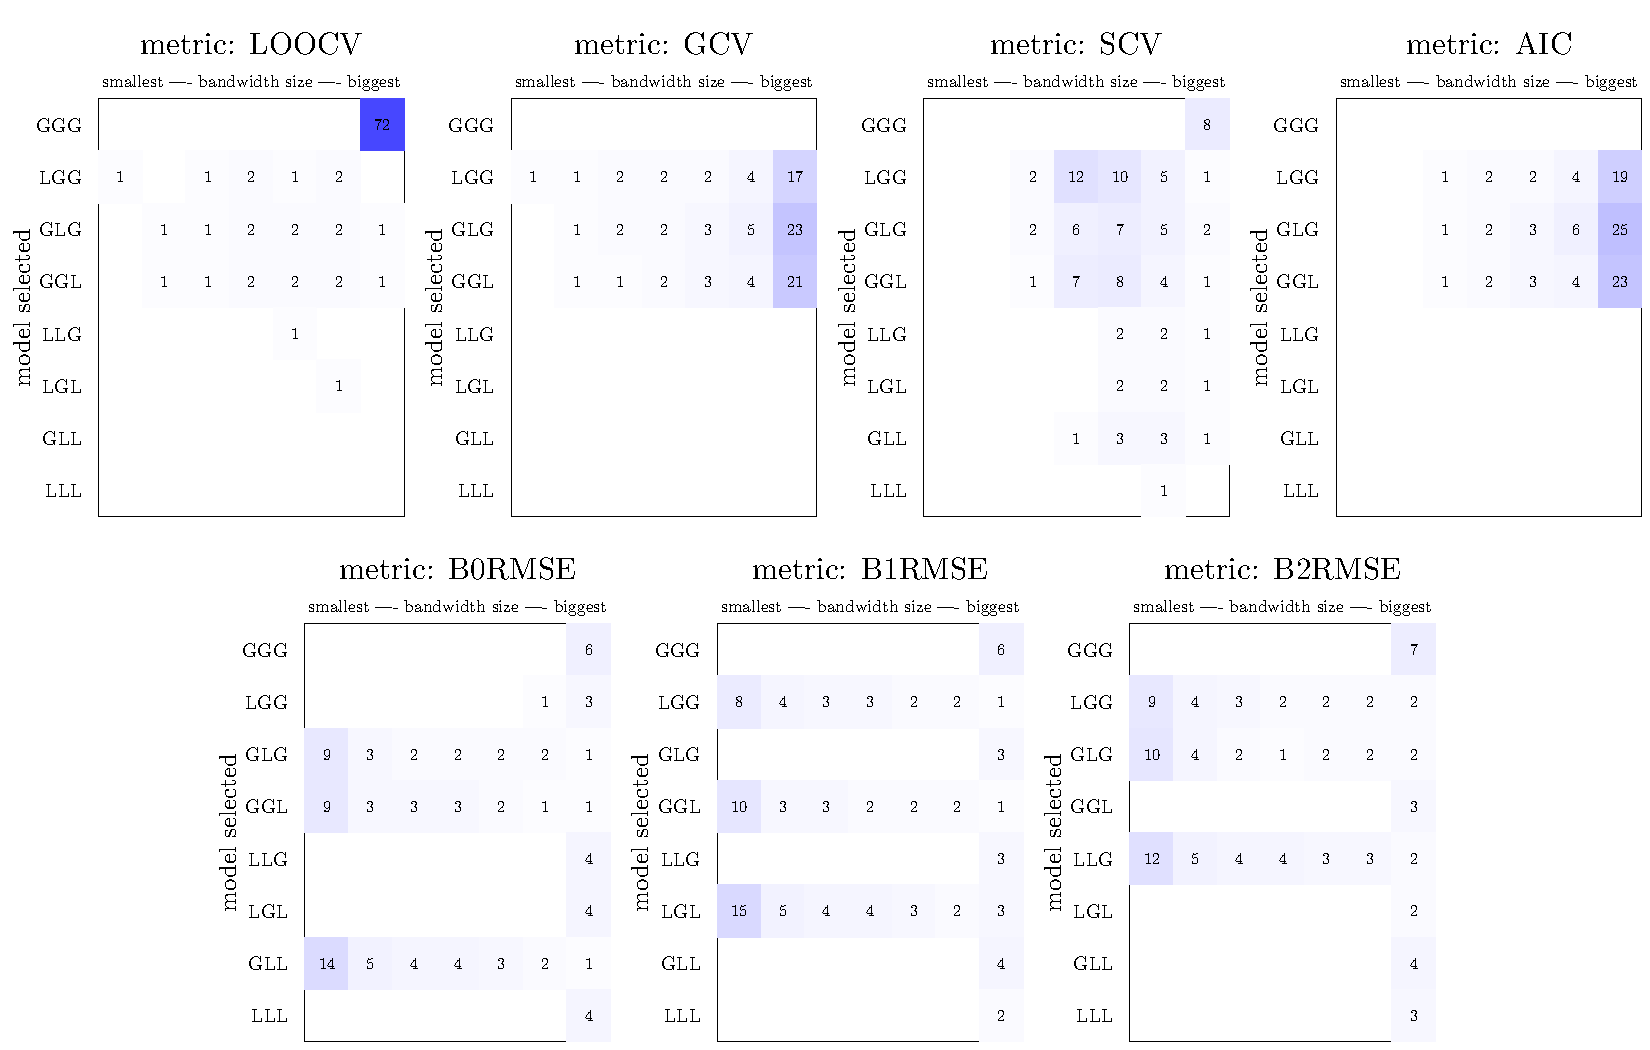
\includegraphics[width = 1.0\textwidth]{figure/BandwidthsGGG.pdf}}
\caption{Model and Bandwidth Selected by Metric when the True Model = `GGG' (All coefficients are stationary) \\ Each subfigure shows the percentage of simulations a given model and bandwidth combination was selected among the 50 possible combinations (7 bandwidths for each of the seven mixed models plus the GGG model) for a given metric. The sum of all values in a given subfigure sum to 100 subject to rounding error. For convenience, cell values less than 0.5 percent are omitted. The color saturation of the cells helps denote the magnitude of the values.}
\label{fig:GGGmodelBandwidths}
\end{sidewaysfigure}

\subsection{All Local Coefficients}

The previous section investigated the simulation results when the true model was stationary across all three coefficients. In this section we examine the opposite extreme: all non-stationary coefficients. To begin, we construct a figure similar to Figure \ref{fig:GGGmodelBandwidths} but with a true model of `LLL.'   



\begin{sidewaysfigure}
  \makebox[\textwidth][c]{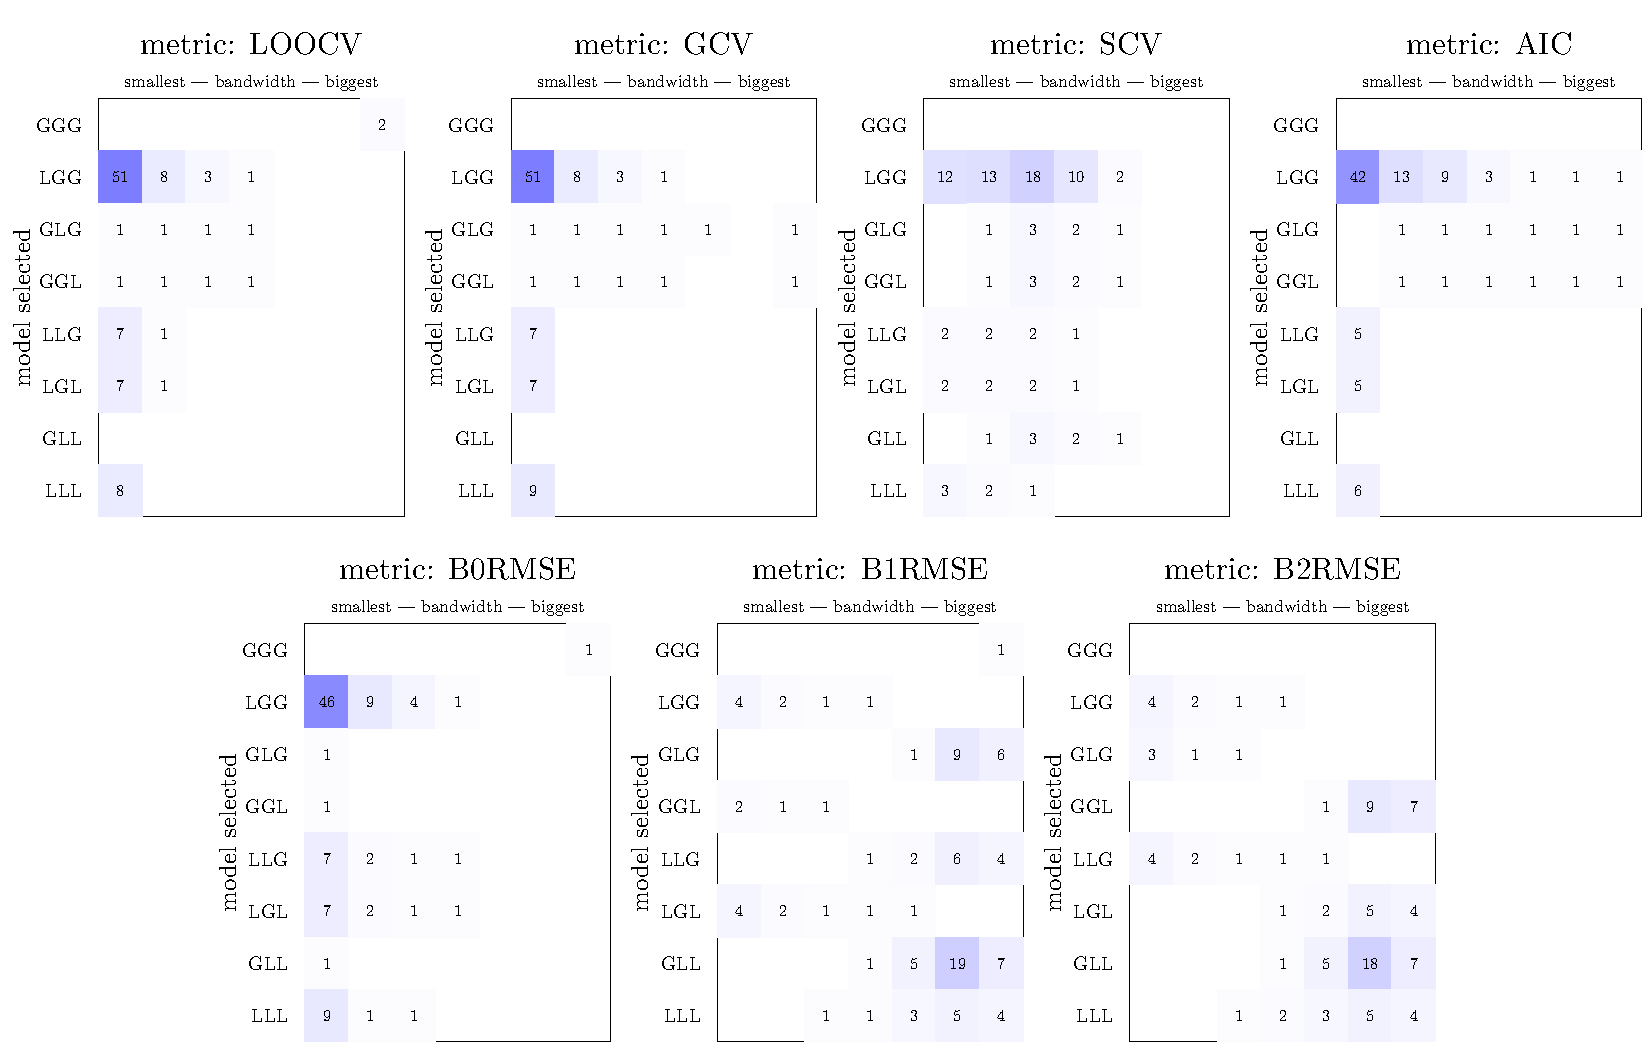
\includegraphics[width = 1.0\textwidth]{figure/ModelBandwidthSelectionLLL.pdf}}
\caption{Model and Bandwidth Selected by Metric when the True Model = `LLL' (All coefficients are non-stationary) \\ Each subfigure shows the percentage of simulations a given model and bandwidth combination was selected among the 50 possible combinations (7 bandwidths for each of the seven mixed models plus the GGG model) for a given metric. The sum of all values in a given subfigure sum to 100 subject to rounding error. For convenience, cell values less than 0.5 percent are omitted. The color saturation of the cells helps denote the magnitude of the values.}
\label{fig:LLLmodelBandwidths}
\end{sidewaysfigure}

Figure \ref{fig:LLLmodelBandwidths} reveals a stark pattern. Although the true underlying model is non-stationary, none of the four metrics choose the `LLL' model in more than 10 percent of our simulations. Instead, the `LGG' model is selected over 50 percent of the time by each metric. The LOOCV, GCV, and AIC metrics all select the `LGG' model with the smallest bandwidth much more frequently than any other model/bandwidth combination. For instance, LOOCV and GCV select the `LGG' model with the smallest bandwidth over 50 percent of the time. 

The second row of results in Figure \ref{fig:LLLmodelBandwidths} displays the model and bandwidth combinations that yield the smallest RMSE for the coefficients in our model. The pattern for the smallest RMSE associated with the intercept term, $\beta _0$ closely resembles the pattern of models and bandwidths for LOOCV, GCC, and AIC. Roughly 10 percent of simulations have the smallest RMSE using the `LLL' model, while roughly half of the simulations selected the `LGG' model with the smallest bandwidth. However, we see a different pattern for $\beta _1$ and $\beta _2$. In both instances, no single model and bandwidth combination yielded the smallest RMSE more than 20 percent of the time (the `GLL' model with the second largest bandwidth). That is, the intercept was fixed while the other two coefficients were treated as non-stationary and the bandwidth was comprised of approximately two-thirds of the observations. 

The simulations contained in Figure \ref{fig:LLLmodelBandwidths} actually contain a lot of variation in the amount of coefficient non-stationarity. Recalling that we implemented two amounts of spatial variation in each coefficient (think of it as `some' and `more') there are actually eight combinations of `LLL' models ranging from ``some, some, some,'' to ``more, more, more.'' We therefore present a comparison of the following three models, the `GGG' model we've already discussed, the `LLL' model containing the smallest amount of overall spatial non-stationarity in all coefficients (the ``some, some, some'' model), and the largest amount of overall spatial non-stationarity (the ``more, more, more'' model).




\begin{figure}
  \makebox[\textwidth][c]{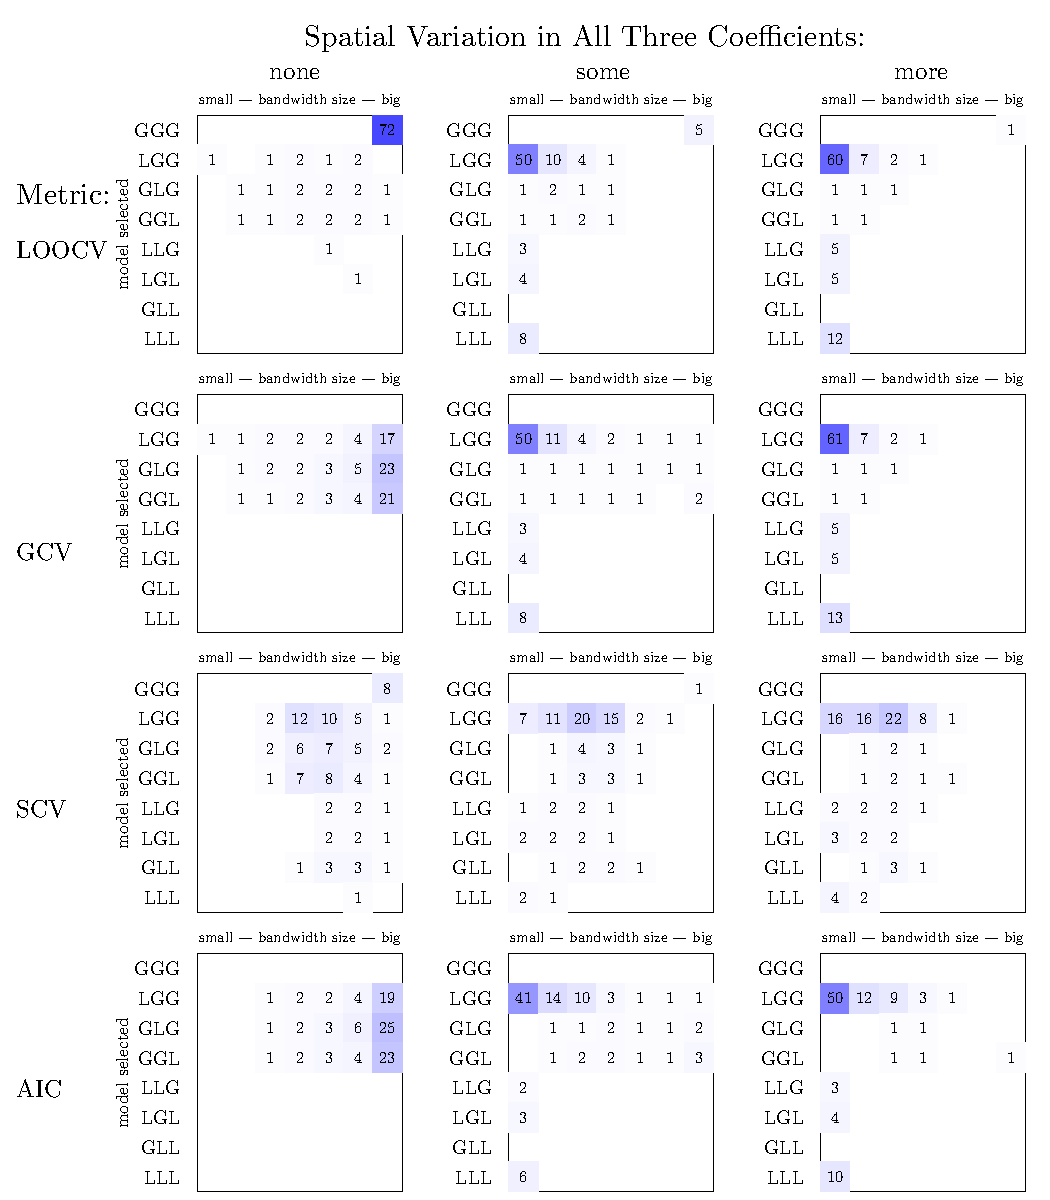
\includegraphics[width = 1.0\textwidth]{figure/ModelSelectionGGGtoLLL.pdf}}
\caption{Model and Bandwidth Selected by Metric for `None', `Some', and `More' Spatial Variation in the Three Regression Coefficients \\ Each subfigure shows the percentage of simulations a given model and bandwidth combination was selected among the 50 possible combinations (7 bandwidths for each of the seven mixed models plus the GGG model) for a given metric. The sum of all values in a given subfigure sum to 100 subject to rounding error. For convenience, cell values less than 0.5 percent are omitted. The color saturation of the cells helps denote the magnitude of the values.}
\label{fig:GGG2LLLmodelBandwidths}
\end{figure}

\subsection{One Local Coefficient}

What have we learned in the previous sections?
\begin{enumerate}
\item LOOCV does the best identifying the non-stationary models
\item most accurate $\hat{\beta}$ estimates do not necessarily come from the correct model
\item SCV sucks
\item something else.
\end{enumerate}

Now we explore the mosed model cases in which some of the coefficients are stationary and some are non-stationary. We begin with the case of a single non-stationary coefficient. 




\begin{sidewaysfigure}
  \makebox[\textwidth][c]{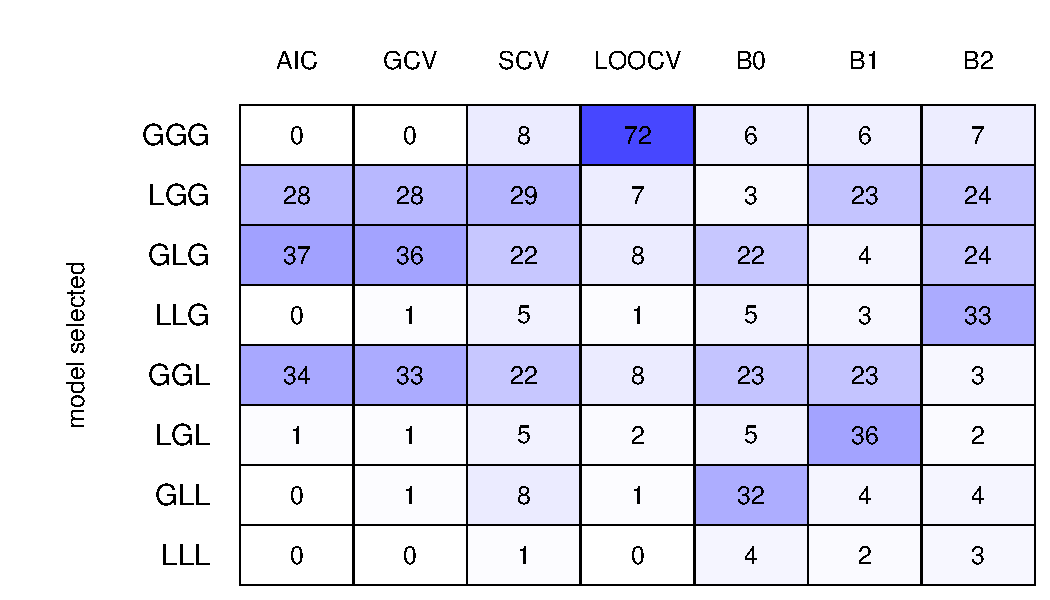
\includegraphics[width = 1.0\textwidth]{figure/ModelSelectionTabulations1.pdf}}
\caption{This figure shows }
\label{fig:modelIdentificationOneL}
\end{sidewaysfigure}

Figure \ref{fig:modelIdentificationOneL} shows that most metrics can correctly identify the propoer mixed model when only one coefficient is non-stationary.

\subsection{Two Local Coefficients}


Now we explore the mixed model cases in which two of the coefficients are non-stationary. 




\begin{sidewaysfigure}
  \makebox[\textwidth][c]{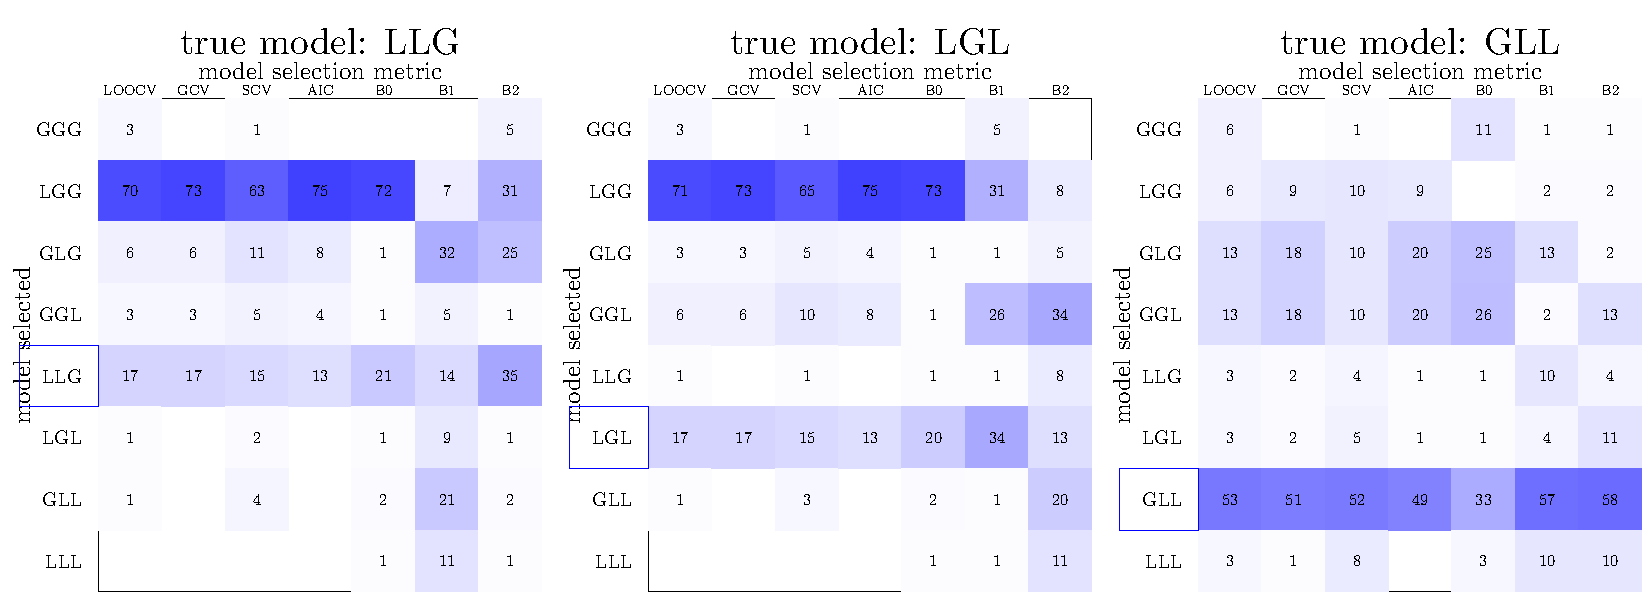
\includegraphics[width = 1.0\textwidth]{figure/ModelSelectionTabulations1G.pdf}}
\caption{This figure shows }
\label{fig:modelIdentificationOneG}
\end{sidewaysfigure}

Figure \ref{fig:modelIdentificationOneG} shows that most metrics can.

\section{Discussion}

Let's show the model selection by metric across our 8 different models.



\begin{figure}
  \makebox[\textwidth][c]{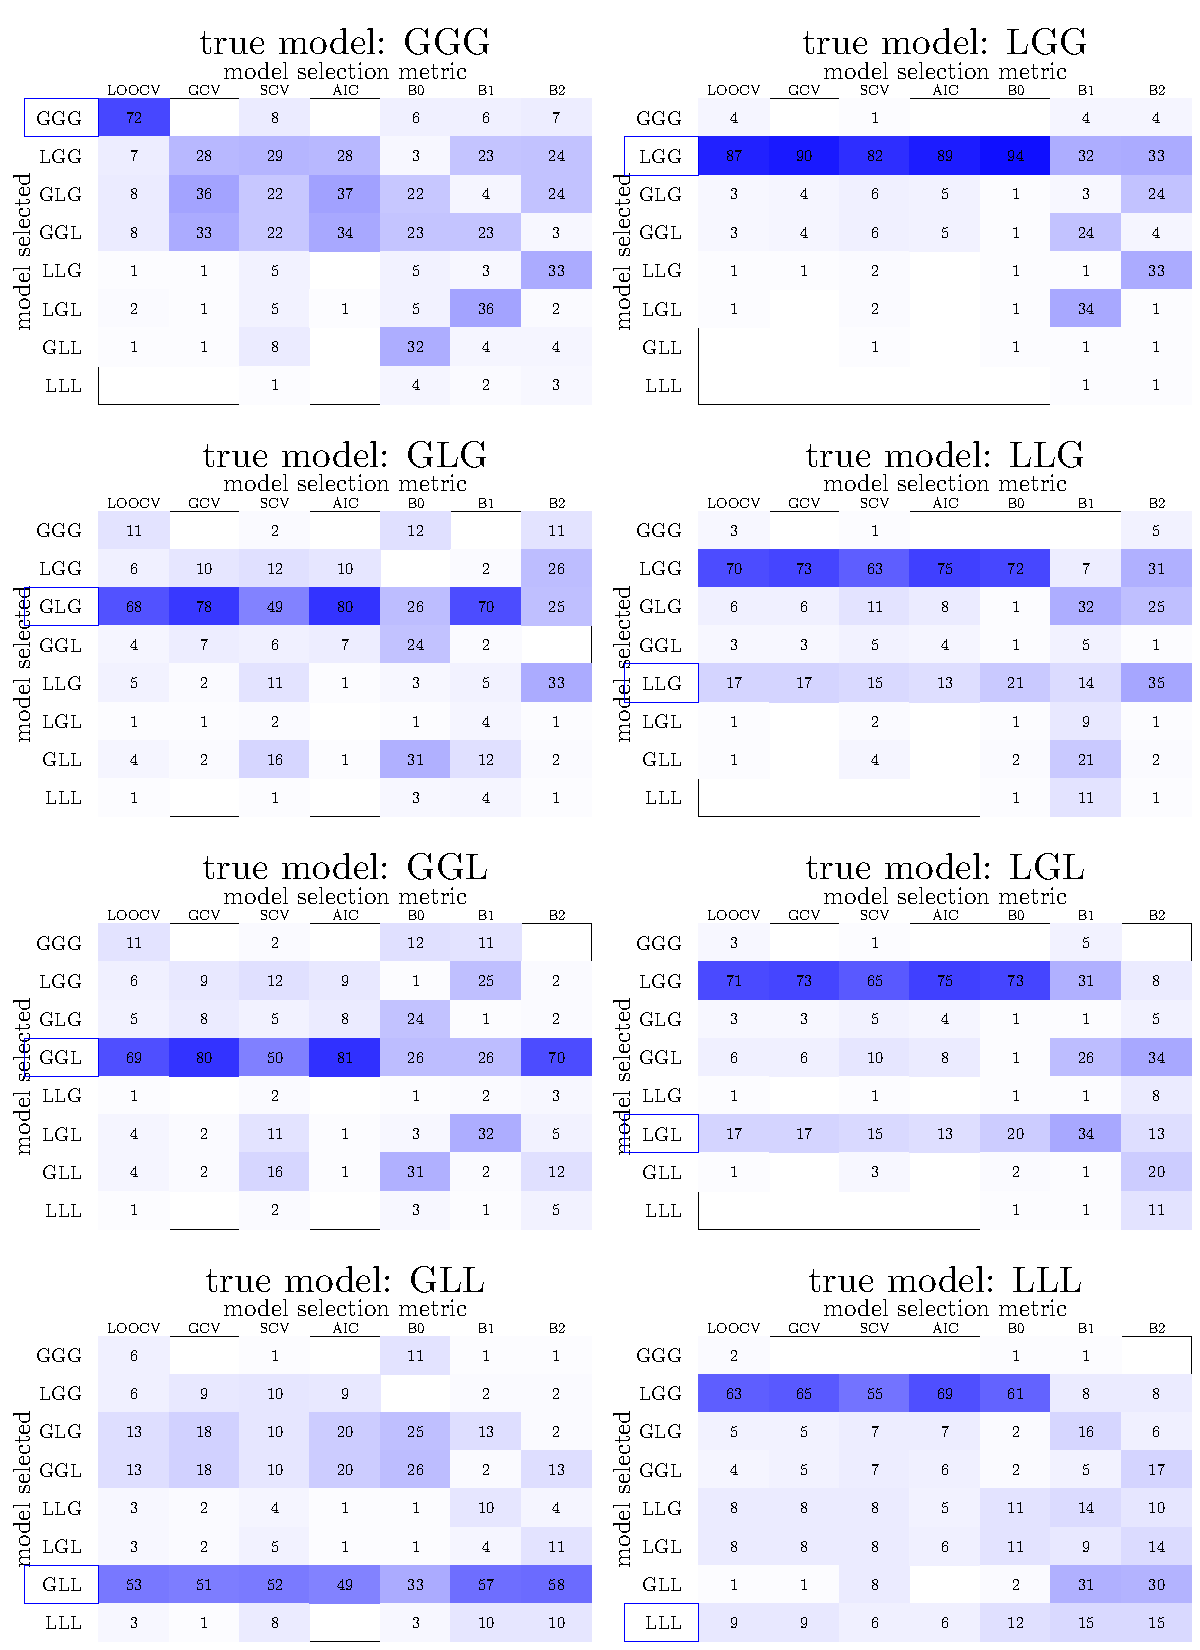
\includegraphics[width = 1.2\textwidth]{figure/ModelSelectionTabulationsAll8.pdf}}
\caption{This figure shows }
\label{fig:modelIdentificationAll8}
\end{figure}

The left (right) column in Figure \ref{fig:modelIdentificationAll8} contains the four models in which the intercept coefficient is (non-)stationary over the study area. In the top row of the figure both $\beta _1$ and $\beta _2$ are stationary, the middle two rows contain one stationary and one non-stationary coefficient, and in the bottom row both $\beta _1$ and $\beta _2$ are non-stationary. An interesting pattern is visible. The models on the left tend to be more accurately identified by the metrics than the models on the right. That is, if the intercept term is stationary, our information metrics do a pretty good job identifying whether or not the other coefficients are stationary or not. However, when the intercept term is stationary, our metrics commonly choose the `LGG' model even when one or both of the other coefficients is non-stationary. 






% \begin{figure}
%   \makebox[\textwidth][c]{\includegraphics[page = 1, width = 1.2\textwidth]{figure/BandwidthsError.pdf}}
% \caption{This figure shows the GLG model...}
% \label{fig:GLGmodelBandwidths}
% \end{figure}
% 
% Figure \ref{fig:GLGmodelBandwidths} shows



% \subsection{Coefficient Formulation}
% 
% Even if an incorrect model is chosen, the model may yield accurate estimates of the coefficients. In each run of the simulation we estimated 50 different model/bandwidth combinations (seven different bandwidths for each of the seven models with at least one coefficient varying over space, plus the standard OLS model). We calculate the Root Mean Squared Error for each model and can rank these values. For instance, it is possible, and often the case, that the ``wrong'' model yields the most accurate estimates of a coefficient among all of the models implemented.
% 
% 
% <<BetaRankTabulations, fig.width=4, fig.height=6, fig.show='animate', aniopts='autoplay,loop,controls', interval=2>>=
% colMat = matrix("black", 8, 3)
% colMat[as.matrix(models)=="yes"] = "red"
% par(oma = c(0, 2, 3, 0))
% par(mar = rep(1, 4))
% for (i in 1:8) {
%   #i = 1
%   layout(matrix(1:12, 4, 3, byrow=T))
%   temp2 = which(mcOutput[1, "True Model", ] == i)
%   inputMetrics = c("AIC", "GCV", "SCV", "LOOCV")
%   inputStats = c("B0RMSE Rank", "B1RMSE Rank", "B2RMSE Rank")
%   for (j in 1:4) {
%     for (k in 1:3) {
%       temp3 = mcOutput[inputMetrics[j], inputStats[k], temp2]
%       #summary(temp3)
%       hist(temp3, xlim = c(0, 50), breaks = 5*(0:10), 
%            col = ifelse(colMat[i, k]=="red", "red", "grey85"),
%        axes = F, ylab = "rel freq", xlab = "rank", main = "")
%     }
%   }
%   mtext(text=paste0("Model #", i, "(non-stationary parameters in red"), 
%         side=3, outer=TRUE, line = 1.8)
%   mtext(inputMetrics, at = seq(.875, .125, length.out=4), side = 2, outer = T)
%   mtext(paste0("B", 0:2), at = seq(.17,.83, length.out=3), 
%         side = 3, outer = T, line = 0, col = colMat[i, ])
% }
% 
% @
% 
% 
% \section{Accuracy of Beta Estimates}
% 
% During the experiment we calculated the Root Mean Squared Error the estimated coefficients for all models. We then ranked each model from smallest to largest RMSEs and collected the RMSE values and ranks for all models that minimized one of the model selection criteria and the model with the smallest RMSE for this coefficient. 
% 
% Let's see if there is a relationship between the RMSE values/ranks and the parameters we modified in the experiment.
% 
% <<makeData>>=
% #   temp2 = which(mcOutput[1, "True Model", ] == i)
% #   inputMetrics = c("AIC", "GCV", "SCV", "LOOCV")
% #   inputStats = c("B0RMSE Rank", "B1RMSE Rank", "B2RMSE Rank")
% # temp3 = mcOutput[inputMetrics[j], inputStats[k], temp2]
% myVars = c("B0RMSE",     "B1RMSE",     "B2RMSE",
%            "B0RMSE Rank",  "B1RMSE Rank",  "B2RMSE Rank", 
%            "Sample Size",  "Error", "True Model",
%            "B0 SpVar", "B1 SpVar", "B2 SpVar", "Model Number")
% rankData1 = as.data.frame(t(mcOutput["AIC", myVars, ]))
% rankData1$Metric = "AIC"
% 
% rankData2 = as.data.frame(t(mcOutput["GCV", myVars, ]))
% rankData2$Metric = "GCV"
% 
% rankData3 = as.data.frame(t(mcOutput["SCV", myVars, ]))
% rankData3$Metric = "SCV"
% 
% rankData4 = as.data.frame(t(mcOutput["LOOCV", myVars, ]))
% rankData4$Metric = "LOOCV"
% 
% rankData = rbind(rankData1, rankData2, rankData3, rankData4)
% 
% rankData$samplesize = rankData[, "Sample Size"]
% rankData$error = as.factor(rankData$Error)
% rankData$truemodel = as.factor(rankData[, "True Model"])
% rankData$B0sv = as.factor(rankData[, "B0 SpVar"])
% rankData$B1sv = as.factor(rankData[, "B1 SpVar"])
% rankData$B2sv = as.factor(rankData[, "B2 SpVar"])
% rankData$metric = as.factor(rankData$Metric)
% names(rankData)[which(names(rankData)=="Model Number")] = "selectedmodel"
% 
% @
% 
% \subsection{RMSE Values}
% 
% <<RMSEregression011>>=
% RMSEregression0 <- lm(B0RMSE ~ samplesize + metric + B0sv + B1sv + B2sv + error, 
%                data = rankData)
% summary(RMSEregression0)
% @
% <<RMSEregression111>>=
% RMSEregression1 <- lm(B1RMSE ~ samplesize + metric + B0sv + B1sv + B2sv + error, 
%                data = rankData)
% summary(RMSEregression1)
% @
% <<RMSEregression211>>=
% RMSEregression2 <- lm(B2RMSE ~ samplesize + metric + B0sv + B1sv + B2sv + error, 
%                data = rankData)
% summary(RMSEregression2)
% @
% 
% Now I'd like to add a variable along the lines of ``does the selected model correctly identify whether the variable is non-stationary?''
% 
% <<identifySV>>=
% TrueModelBeta0sv = c(2, 4, 6, 8)
% TrueModelBeta1sv = c(3, 4, 7, 8)
% TrueModelBeta2sv = 5:8
% 
% ModelBetaSV.selected.true = function(TrueModelBetasv) {
%   temp = rankData$truemodel %in% TrueModelBetasv
%   temp2 = rankData$selectedmodel %in% TrueModelBetasv
%   ModelBetaSVCorrect <- temp == temp2
%   ModelBetaSVCorrect
% }
% 
% rankData$ModelBeta0svTrue = ModelBetaSV.selected.true(TrueModelBeta0sv)
% rankData$ModelBeta1svTrue = ModelBetaSV.selected.true(TrueModelBeta1sv)
% rankData$ModelBeta2svTrue = ModelBetaSV.selected.true(TrueModelBeta2sv)
% @
% 
% <<RMSEregression012>>=
% RMSEregression0 <- lm(B0RMSE ~ samplesize + metric + B0sv + B1sv + B2sv + error + ModelBeta0svTrue, 
%                data = rankData)
% summary(RMSEregression0)
% @
% <<RMSEregression112>>=
% RMSEregression1 <- lm(B1RMSE ~ samplesize + metric + B0sv + B1sv + B2sv + error + ModelBeta1svTrue, 
%                data = rankData)
% summary(RMSEregression1)
% @
% <<RMSEregression212>>=
% RMSEregression2 <- lm(B2RMSE ~ samplesize + metric + B0sv + B1sv + B2sv + error + ModelBeta2svTrue, 
%                data = rankData)
% summary(RMSEregression2)
% @
% 
% Now add all three:
% 
% <<RMSEregression013>>=
% RMSEregression0 <- lm(B0RMSE ~ samplesize + metric + B0sv + B1sv + B2sv + error + ModelBeta0svTrue, 
%                data = rankData)
% summary(RMSEregression0)
% @
% <<RMSEregression113>>=
% RMSEregression1 <- lm(B1RMSE ~ samplesize + metric + B0sv + B1sv + B2sv + error + ModelBeta1svTrue, 
%                data = rankData)
% summary(RMSEregression1)
% @
% <<RMSEregression213>>=
% RMSEregression2 <- lm(B2RMSE ~ samplesize + metric + B0sv + B1sv + B2sv + error + ModelBeta2svTrue, 
%                data = rankData)
% summary(RMSEregression2)
% @
% 
% \subsection{RMSE Rank}
% How are the various parameters related to the results of the $\beta _0$ ranking?
% <<regression021>>=
% rankData$B0rank = rankData[, "B0RMSE Rank"]
% rankData$B1rank = rankData[, "B1RMSE Rank"]
% rankData$B2rank = rankData[, "B2RMSE Rank"]
% rankLM <- lm(B0rank ~ samplesize + metric + B0sv + B1sv + B2sv + error, 
% data = rankData)
% summary(rankLM)
% @
% 
% How are the various parameters related to the results of the $\beta _1$ ranking?
% <<regression121>>=
% rankLM <- lm(B1rank ~ samplesize + metric + B0sv + B1sv + B2sv + error, data = rankData)
% summary(rankLM)
% @
% 
% How are the various parameters related to the results of the $\beta _2$ ranking?
% <<regression221>>=
% rankLM <- lm(B2rank ~ samplesize + metric + B0sv + B1sv + B2sv + error, data = rankData)
% summary(rankLM)
% @
% 
% 
% Now add in whether or not the correct model was specified.
% <<regression022>>=
% rankLM <- lm(B0rank ~ samplesize + metric + B0sv + B1sv + B2sv + error + ModelBeta0svTrue, data = rankData)
% summary(rankLM)
% @
% 
% How are the various parameters related to the results of the $\beta _1$ ranking?
% <<regression122>>=
% rankLM <- lm(B1rank ~ samplesize + metric + B0sv + B1sv + B2sv + error + ModelBeta1svTrue, data = rankData)
% summary(rankLM)
% @
% 
% How are the various parameters related to the results of the $\beta _2$ ranking?
% <<regression222>>=
% rankLM <- lm(B0rank ~ samplesize + metric + B0sv + B1sv + B2sv + error + ModelBeta2svTrue, data = rankData)
% summary(rankLM)
% @
% 
% Let's also throw in all three variables about whether the selected model has the same spatial variation as the true model for a certain beta.
% 
% <<regression023>>=
% rankLM <- lm(B0rank ~ samplesize + metric + B0sv + B1sv + B2sv + error + ModelBeta0svTrue+ ModelBeta1svTrue+ ModelBeta2svTrue, data = rankData)
% summary(rankLM)
% @
% 
% How are the various parameters related to the results of the $\beta _1$ ranking?
% <<regression123>>=
% rankLM <- lm(B1rank ~ samplesize + metric + B0sv + B1sv + B2sv + error + ModelBeta0svTrue+ ModelBeta1svTrue+ ModelBeta2svTrue, data = rankData)
% summary(rankLM)
% @
% 
% How are the various parameters related to the results of the $\beta _2$ ranking?
% <<regression223>>=
% rankLM <- lm(B2rank ~ samplesize + metric + B0sv + B1sv + B2sv + error + ModelBeta0svTrue+ ModelBeta1svTrue+ ModelBeta2svTrue, data = rankData)
% summary(rankLM)
% @
% 
% \subsection{RMSE Rank Proportion}
% 
% Let's convert ranks into a proportion and then use a logistic regression to look for patterns in rank vs.\ other variables like the metric and degree of spatial variation, etc.
% 
% How are the various parameters related to the results of the $\beta _0$ ranking?
% <<regression031>>=
% rankData$B0rankP = rankData[, "B0RMSE Rank"]/50
% rankData$B1rankP= rankData[, "B1RMSE Rank"]/50
% rankData$B2rankP = rankData[, "B2RMSE Rank"]/50
% mylogit <- glm(cbind(B0rankP, 1-B0rankP) ~ samplesize + metric + B0sv + B1sv + B2sv + error, 
% data = rankData, family = "binomial")
% summary(mylogit)
% @
% 
% How are the various parameters related to the results of the $\beta _1$ ranking?
% <<regression131>>=
% mylogit <- glm(cbind(B1rankP, 1-B1rankP) ~ samplesize + metric + B0sv + B1sv + B2sv + error, 
% data = rankData, family = "binomial")
% summary(mylogit)
% @
% 
% How are the various parameters related to the results of the $\beta _2$ ranking?
% <<regression231>>=
% mylogit <- glm(cbind(B2rankP, 1-B2rankP) ~ samplesize + metric + B0sv + B1sv + B2sv + error, 
% data = rankData, family = "binomial")
% summary(mylogit)
% @
% 
% 
% Now add in whether the model selected a model with appropriate spatial variation for the parameter.
% <<regression032>>=
% mylogit <- glm(cbind(B0rankP, 1-B0rankP) ~ samplesize + metric + B0sv + B1sv + B2sv + error + ModelBeta0svTrue, 
% data = rankData, family = "binomial")
% summary(mylogit)
% @
% 
% How are the various parameters related to the results of the $\beta _1$ ranking?
% <<regression132>>=
% mylogit <- glm(cbind(B1rankP, 1-B1rankP) ~ samplesize + metric + B0sv + B1sv + B2sv + error + ModelBeta1svTrue, 
% data = rankData, family = "binomial")
% summary(mylogit)
% @
% 
% How are the various parameters related to the results of the $\beta _2$ ranking?
% <<regression232>>=
% mylogit <- glm(cbind(B2rankP, 1-B2rankP) ~ samplesize + metric + B0sv + B1sv + B2sv + error + ModelBeta2svTrue, 
% data = rankData, family = "binomial")
% summary(mylogit)
% @
% 
% Let's also throw in all three variables about whether the selected model has the same spatial variation as the true model for a certain beta.
% 
% <<regression033>>=
% mylogit <- glm(cbind(B0rankP, 1-B0rankP) ~ samplesize + metric + B0sv + B1sv + B2sv + error + ModelBeta0svTrue+ ModelBeta1svTrue+ ModelBeta2svTrue, 
%                data = rankData, family = "binomial")
% summary(mylogit)
% @
% 
% How are the various parameters related to the results of the $\beta _1$ ranking?
% <<regression133>>=
% mylogit <- glm(cbind(B1rankP, 1-B1rankP) ~ samplesize + metric + B0sv + B1sv + B2sv + error + ModelBeta0svTrue+ ModelBeta1svTrue+ ModelBeta2svTrue, 
%                data = rankData, family = "binomial")
% summary(mylogit)
% @
% 
% How are the various parameters related to the results of the $\beta _2$ ranking?
% <<regression233>>=
% mylogit <- glm(cbind(B2rankP, 1-B2rankP) ~ samplesize + metric + B0sv + B1sv + B2sv + error + ModelBeta0svTrue+ ModelBeta1svTrue+ ModelBeta2svTrue, 
%                data = rankData, family = "binomial")
% summary(mylogit)
% @

\newpage
\begin{singlespace}
\bibliographystyle{plainnat}
\bibliography{MixedGWRbibliography}
\end{singlespace}

\end{document}
